% Chapter Template

\chapter{Charakterystyka kwadrokopterów} % Main chapter title

\label{Chapter2} % Change X to a consecutive number; for referencing this chapter elsewhere, use \ref{ChapterX}

\lhead{Chapter 2. \emph{Charakterystyka kwadrokopterów}} % Change X to a consecutive number; this is for the header on each page - perhaps a shortened title

%----------------------------------------------------------------------------------------
%	SECTION 1
%----------------------------------------------------------------------------------------

\section{Zasada działania}
Kwadrokopter zaliczany jest do rodziny śmigłowców, czyli statków powietrznych wytwarzających siłę nośną dzięki ruchowi obrotowemu wirników (rys.~\ref{fig:quadrotor_clasification.png})  [wikipedia, 6.pdf, 8.pdf[4] str 172]. Kwadrokoptery różnią się nieco od konstrukcji klasycznego helikoptera - posiadają cztery wirniki umieszczone poziomo, które wirują parami w przeciwne strony (dwa wirniki zgodnie z ruchem wskazówek zegara, dwa przeciwnie do ruchu wskazówek zegara). Dzięki obrotom śmigieł w przeciwnych kierunkach momenty bezwładności, próbujące obrócić kwadrokopter wokół własnej osi znoszą się, a co za tym idzie w tego typu konstrukcjach nie trzeba stosować wirnika ogonowego. Pociąga to za sobą w konsekwencji bardzo prostą konstrukcję mechaniczną oraz lepszą w porównaniu do helikopterów manewrowość. 

\begin{figure}[htbp]
	\centering
		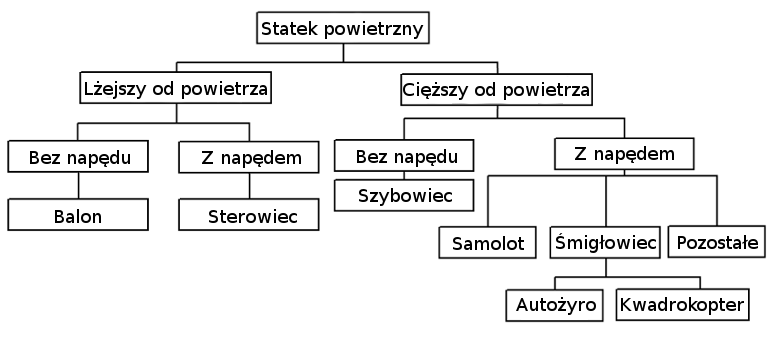
\includegraphics[width=0.8\textwidth]{Pictures/quadrotor_clasification2.png}
		%\rule{35em}{0.5pt}
		\caption[Klasyfikacja statków powietrznych]{Klasyfikacje statków powietrznych}
		\label{fig:quadrotor_clasification.png}
\end{figure}

Do opisu ruchu i położenia kwadrokoptera wprowadza się dwa układy odniesienia: inercjalny układ odniesienia (np. układ współrzędnych pilota kwadrokoptera, zwany często układem współrzędnych Ziemi) oraz układ odniesienia kwadrokoptera [6,7,9,11]. Przy tak zdefinowanych układach odniesienia możemy określić trzy kąty (rys.~\ref{fig:quadrotor_frames.png}):

\begin{itemize}
	\item Kąt przechylenia (ang. Roll) \straightphi: jest to kąt obrotu wokół osi Xb || Xe
	\item Kąt pochylenia (ang. Pitch) \straighttheta: jest to kąt obrotu wokół osi Yb || Ye 
	\item Kąt odchylenia (ang. Yaw) \textpsi: jest to kąt obrotu wokół osi Zb || Ze
\end{itemize}

\begin{figure}[!htb]
	\centering
		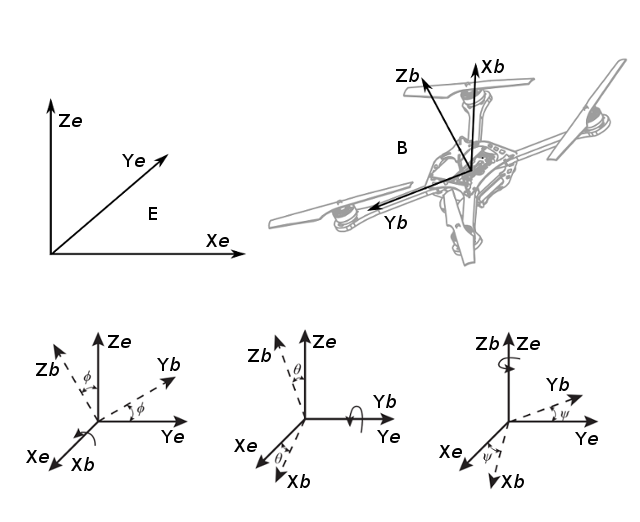
\includegraphics[width=0.7\textwidth]{Pictures/quadrotor_frames.png}
		%\rule{35em}{0.5pt}
		\caption[Układy odniesienia]{Układ odniesienia zewnętrznego obserwatora E (inercjalny układ odniesienia) oraz układ odniesienia kwadrokoptera B, wraz z zaznaczonymi kątami\,przechylenia\,(\straightphi), pochylenia (\straighttheta) oraz odchylenia (\textpsi) (konfiguracja ,,+'')}
	\label{fig:quadrotor_frames.png}
\end{figure}

Kąty (\straightphi,\straighttheta,\textpsi) zwane są kątami Eulera i służą do opisu przejścia między układem odniesienia Ziemi a układem odniesienia kwadrokoptera.

Chcąc zrozumieć w jaki sposób można osiągnąć ruch liniowy oraz obrotowy kwadrokoptera, należy spojrzeć na siły i momenty sił, które na niego działają (rys.~\ref{fig:quadrotor_forces}). 

\begin{figure}[H]
	\centering
		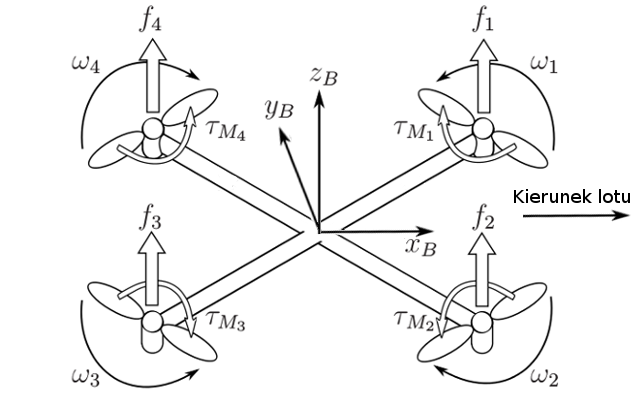
\includegraphics[width=0.62\textwidth]{Pictures/quadrotor_forces.png}
		%\rule{35em}{0.5pt}
		\caption[Siły i momenty sił działające na kwadrokopter]{Siły i momenty sił działające na kwadrokopter (konfiguracja ,,X'')}
	\label{fig:quadrotor_forces}
\end{figure}


Na kwadrokopter (pomijając siłę grawitacji) działają cztery siły ciągów silników $\mathnormal{f_1, f_2, f_3, f_4}$, oraz cztery momenty sił $\tau_{M_1}, \tau_{M_2}, \tau_{M_3}, \tau_{M_4}$, gdzie $\tau_{M_i}$ jest momentem reakcji silnika, spowodowawnym oporem aerodynamicznym śmigieł [odniesienia do bibliografii] . 
Siła unosząca kwadrokopter w powietrzu jest sumą sił ciągu wszystkich silników. Moment siły, obracający kwadrokopter wokół osi Xb (powodujący przechylenie) jest wynikiem różnicy (f1+f4) - (f2+f3), natomiast moment siły obracający kwadrokopter wokół osi Yb (powodujący pochylenie) jest wynikiem różnicy (f1+f2) - (f3 + f4). 
Moment siły obracający kwadrokopter wokół osi Zb (powodujący odchylenie) jest wynikiem sumy $\tau_{M_1} + \tau_{M_2} + \tau_{M_3} + \tau_{M_4}$.  Zmieniając wartości tych sił i momentów można kontrolować ruch liniowy kwadrokoptera we wszystkich kierunkach jak również ruch obrotowy wokół każdej z jego osi. Warto zauważyć że siły ciągu silników oraz momenty sił działające na quadrocopter wynikają (przy założeniu że skok łopat śmigieł się nie zmienia) bezpośrednio z prędkości kątowej wirników $\mathnormal{\omega_1, \omega_2, \omega_3, \omega_4}$. Dzięki temu zmieniając jedynie prędkości obrotowe wirników, co jest bardzo proste do osiągnięcia za pomocą elektronicznych sterowników, zyskujemy pełną kontrolę nad wszystkimi sześcioma stopniami swobody kwadrokoptera.  

Mając świadomość sił działających na kwadrokopter możemy napisać warunki równowagi oraz ruchu:

\begin{itemize}
	\item \textbf{Warunek zawisu w powietrzu}\\ Równowaga sił: $\sum_{i=1}^{4} f_i = mg$ \\ Zgodność kierunków: $f_1,_2,_3,_4 \parallel mg$ \\Równowaga momentów: $ \tau_{M_1} + \tau_{M_3} = \tau_{M_2} + \tau_{M_4}$ \\ Równowaga prędkości kątowych: $\omega_1 + \omega_3 = \omega_2 + \omega_4$ \\ 
	\item \textbf{Warunek ruchu w pionie} \\ \textbf{Brak równowagi sił: $\sum_{i=1}^{4} f_i \neq mg$} \\ Zgodność kierunków: $f_1,_2,_3,_4 \parallel mg$ \\ Równowaga momentów: $\tau_{M_1} + \tau_{M_3} = \tau_{M_2} + \tau_{M_4}$ \\ Równowaga prędkości kątowych: $\omega_1 + \omega_3 = \omega_2 + \omega_4$ \\ 
	\item \textbf{Warunek ruchu poziomego} \\ \textbf{Brak równowagi sił: $\sum_{i=1}^{4} f_i \neq  mg$} \\ \textbf{Brak zgodność kierunków: $f_1,_2,_3,_4 \not\parallel mg$} \\ Równowaga momentów: $\tau_{M_1} + \tau_{M_3} = \tau_{M_2} + \tau_{M_4}$ \\ \textbf{Brak równowagi prędkości kątowych: $\omega_1 + \omega_2 \neq  \omega_3 + \omega_4$ lub $\omega_1 + \omega_4 \neq \omega_2 + \omega_3$}\\ 
	\item \textbf{Warunek obrotu wokół własnej osi (osi pionowej Zb)} \\ Równowaga sił: $\sum_{i=1}^{4} f_i = mg$ \\ Zgodność kierunków: $f_1,_2,_3,_4 \parallel mg$ \\ \textbf{Brak równowagi momentów: $\tau_{M_1} + \tau_{M_3} \neq \tau_{M_2} + \tau_{M_4}$}\\ \textbf{Brak równowagi prędkości kątowych: $\omega_1 + \omega_3 \neq  \omega_2 + \omega_4$} \\ 

\end{itemize}

Warunek swobodnego zawisu w powietrzu jest najprostszy do rozpatrzenia: kwadrokopter będzie wisiał nieruchomo, gdy siły ciągu wszystkich czterech wirników będą działać pionowo w górę równoważąc jednocześnie siłę ciężkości, z jaką Ziemia przyciąga kwadrokopter. Dzięki temu że, sumy par prędkości obrotowych śmigieł kręcących się w przeciwne strony są sobie równe, momenty sił, próbujące obrócić kwadrokopter wokół własnej osi znoszą się.

Warunek ruchu w pionie różni się od warunku swobodnego zawisu w powietrzu jedynie tym, że siły ciągu silników nadal są równoległe do siły ciężkości, ale jej nie równoważą. Uzyskuje się to przez równomierne zwiększenie lub zmniejszenie prędkości obrotowych wszystkich wirników. Możemy zatem rozróżnić warunek ruchu w górę: $\sum_{i=1}^{4} f_i > mg$, oraz warunek ruchu w dół: $\sum_{i=i}^{4} fi < mg$.

Warunek obrotu wokół własnej osi uzyskuje się przez zwiększenie prędkości kątowych pary śmigieł (np. smigieł obracających się zgodnie z ruchem wskazówek zegara) i jednoczesne zmniejszenie prędkości pary śmigieł obracających się w przeciwnym kierunku. Dzięki temu momenty sił przestają się równoważyć i kwadrokopter zaczyna obracać sie wokół własnej osi.

Najciekawszym przypadkiem do rozpatrzenia jest warunek ruchu poziomego. Aby kwadrokopter zaczął poruszać się wzdłuż osi $Xe$ lub $Ye$ należy odpowiednio zmienić prędkości kątowe wirników tak, aby nastąpił obrót kwadrokoptera wokół osi odpowiednio $Yb$ lub $Xb$. Chcąc przykładowo uzyskać obrót wokół osi $Xb$ (rys.~\ref{fig:quadrotor_forces}), należy zwiększyć prędkości kątowe wirników 1 oraz 4, zmniejszając jednocześnie prędkości wirników 2 i 3. Dzięki temu powstaje moment obrotowy wokół osi $Xb$, powodujący przechylenie kwadrokoptera. Wypadkowa siła ciągu wszystkich silników nie działa już pionowo ku górze, przez co kwadrokopter zaczyna poruszać sie w poziomie. 

\begin{figure}[H]
	\centering
	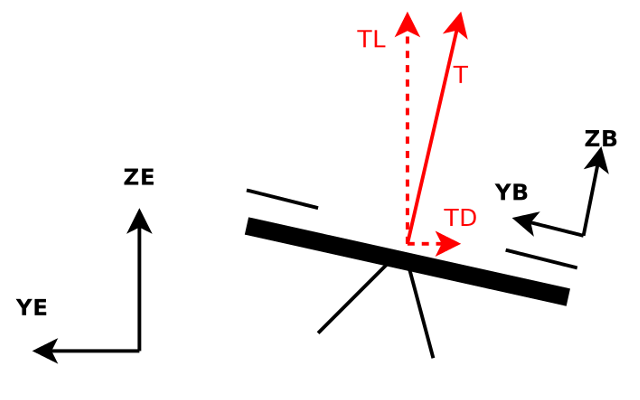
\includegraphics[width=0.7\textwidth]{Pictures/quadrotor_drag_force.png}
		%\rule{35em}{0.5pt}
	\caption[Dynamika ruchu postępowego]{Siły działające na kwadrokopter w trakcie ruchu postępowego}
	\label{fig:quadrotor_drag_force.png}
\end{figure}


Jak widać na rysunku~\ref{fig:quadrotor_drag_force.png}, w trakcie ruchu postępowego siła ciągu każdego wirnika dzieli się na dwie składowe - pionową i poziomą. Składowa pionowa ma na celu zrównoważenie siły grawitacji, natomiast składowa pozioma zapewnienia ruch w poziomie. Warto zwrócić tu uwagę, że przy ruchu poziomym kwadrokoptera należy zwiększyć ciąg silników tak, aby składowa pionowa ciągu silnika nadal równoważyła siłę grawitacji.

W zależności od ustawienia wirników względem układu współrzędnych kwadrokoptera rozróżniamy jego dwie podstawowe konfiguracje - konfiguracja ''+''  oraz konfiguracja ''X'' (Odniesienia do bibliografii)

\begin{figure}[htbp]
	\centering
		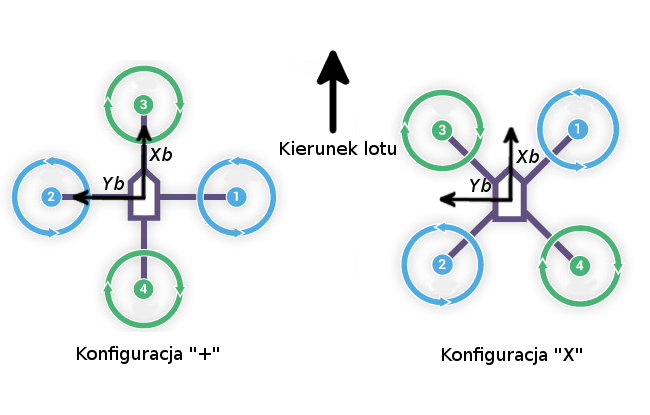
\includegraphics[width=0.7\textwidth]{Pictures/quadrotor_configurations.png}
		%\rule{35em}{0.5pt}
	\caption[Konfiguracje kwadrokopterów]{Konfiguracje ustawień wirników względem osi kwadrokoptera}
	\label{fig:quadrotor_configurations.png}
\end{figure}

W przypadku konfiguracji ''+'' wirniki 1 oraz 2 umieszczone są na osi $Y_b$, natomiast wirniki 3 i 4 na osi $X_b $. Chcąc uzyskać ruch wzdłuż osi $X_e$ lub $Y_e$ należy zmienić prędkości obrotowe jedynie dwóch silników, podczas gdy prędkości obrotowe pozostałych dwóch pozostają bez zmian. Sprawia to, że algorytm kontrolujący ruch kwadrokoptera jest prostszy niż dla konfiguracji ''X''. W konfiguracji ''X'' każdy z wirników leży pomiędzy osiami $X_b$ i $Y_b$ kwadrokoptera. W związku z tym, ruch wzdłuż osi $X_e$ lub $Y_e$ odbywa się dzięki zmianie prędkości obrotowych wszystkich wirników jednocześnie. Sprawia to, że algorytm sterujący będzie trudniejszy w implementacji, lecz niesie ze sobą jedną zaletę - chcąc uzyskać obrót kwadrokoptera np. wokół osi $X_b$ przy konfiguracji ''X'' potrzebna będzie dwa razy mniejsza zmiana prędkości obrotowej każdego z czterech wirników niż dla konfiguracji ''+'' gdzie przy obrocie będą brały udział jedynie silniki 1 i 2. Dzięki temu konfiguracja ''X'' dużo lepiej sprawdza się w sytuacjach, gdzie silniki pracują blisko granicy maksymalnych obrotów (granicy nasycenia) [odniesienie do bibliografii].
%----------------------------------------------------------------------------------------
%	SECTION 2
%----------------------------------------------------------------------------------------

\section{Podstawowe podzespoły}

W podstawowej konfiguracji system sterowania kwadrokopterem można podzielić na następujące moduły:
\begin{itemize}
	\item{kontroler lotu}
	\item{moduł czujników}
	\item{moduł komunikacyjny}
	\item{sterowniki silników}
	\item{silniki}
\end{itemize}

\begin{figure}[H]
	\centering
		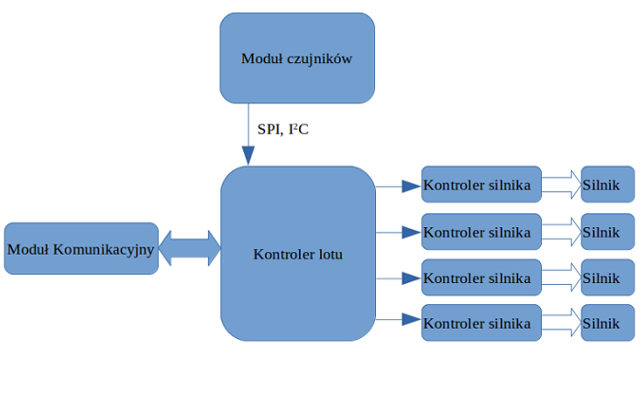
\includegraphics[width=0.7\textwidth]{Pictures/quadrotor_modules.png}
		%\rule{35em}{0.5pt}
	\caption[Podstawowe moduły kwawdrokoptera]{Podstawowe elementy składowe systemu sterowania kwadrokopterem}
	\label{fig:quadrotor_modules.png}
\end{figure}

\subsection{Kontroler lotu}

Kontroler lotu jest podstawowym modułem kwadrokoptera, odpowiedzialnym za stabilizację lotu oraz wykonywanie wszelkich manewrów. Składa się on zazwyczaj z mikrokontrolera wyposażonego w szeregowe lub równoległe interfejsy komunikacyjne, które umożliwiają odbieranie danych z modułu czujników oraz modułu komunikacyjnego, jak również przesyłanie danych do kontrolerów silników. Duża różnorodność obecnie dostępnych mikrokontrolerów sprawia, że można zaobserwować najrozmaitsze konstrukcje kontrolerów oparte o takie architektury jak AVR lub ARM, od własnoręcznie robionych płytek drukowanych po gotowe komputery jednopłytkowe (SBC), w tym ostatnio raspberry PI [odniesienia do bibliografii]. W dziedzinie dostepnego oprogramowania również widoczna jest duża różnorodność. Wśród najbardziej popularnych rozwiązań wyróżnić można programy dedykowane do kontroli lotu, takie jak ArduPilot (odniesienie do bibliografii), programy napisane w oparciu o proste systemy operacyjne czasu rzeczywistego (RTOS) (odniesienie do bibliografii), a także programy oparte o specjalne dystrybucje systemu LINUX (Parrot, odniesienie do bibliografii).

\subsection{Moduł czujników}

Moduł czujników służy do zbierania informacji niezbędnych kontrolerowi lotu do utrzymania stabilizacji kwadrokoptera, jak również wykonywania odpowiednich manewrów. W ostatnich latach dzięki rozwojowi technologii MEMS (odniesienia do bibliografii) dostępne stały się układy scalone ze zintegrowanymi czujnikami, posiadające cyfrowe lub analogowe interfejsy komunikacyjne, zwane również IMU (ang. Inertial Measurement Unit) (odniesienie do bibliografii). W najprostszej konfiguracji układy scalone wyposażone są w trzyosiowy akcelerometr i trzyosiowy żyroskop, dzięki czemu zapewniają komplet informacji potrzebnych dla kontrolera lotu. Niektóre moduły czujników oferują również sprzętową akcelerację obliczeń (odniesienia do noty katalogowej MPU-6050), zwalniając tym samym kontroler lotu z konieczności przeliczania położenia kwadrokoptera w przestrzeni. 

\subsection{Moduł komunikacyjny}

Moduł komunikacyjny realizuje komunikację między pilotem a quadrokopterem. Obecnie najbardziej popularna droga komunikacji to droga radiowa lecz w tańszych konstrukcjach można spotkać jednostronną komunikację wykorzystującą promieniowanie podczerwone. Wśród prywatnych konstrukcji kwadrokopterów często można spotkać moduły radiowe pracujące w paśmie 2.4GHz lub 434MHz, wyposażone w interfejs SPI, a także znacznie prostsze w obsłudze moduły Bluetooth, których wadą jest znacznie mniejszy zasięg transmisji danych. Wśród gotowych modułów komunikacyjnych dostepnych na rynku najbardziej popularne są moduły pracujące w paśmie 2.4GHz, oferujące kilka analogowych kanałów wyjściowych z modulacją PWM (wikipedia) lub PPM (wikipedia)(http://www.endurance-rc.com/ppmtut.php). 

\begin{figure}[H]
	\centering
		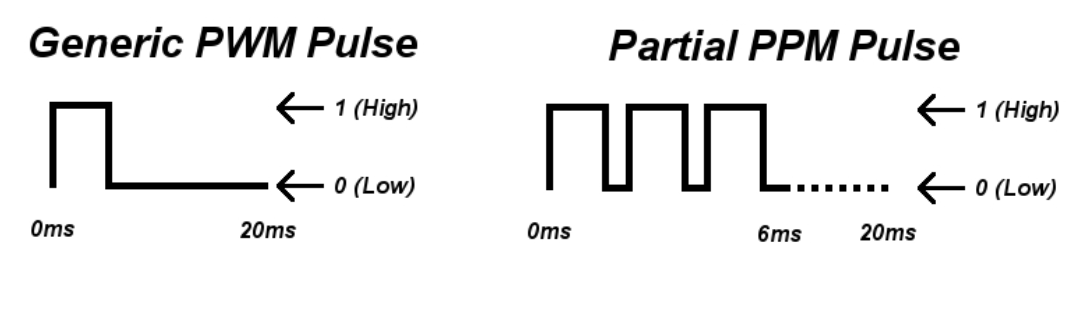
\includegraphics[width=0.7\textwidth]{Pictures/quadrotor_controller_pwm_ppm.png}
		%\rule{35em}{0.5pt}
	\caption[Przykłady modulacji w modelarstwie]{Przykłady modulacji PWM i PPM używanych najczęściej w modelarstwie}
	\label{fig:quadrotor_modules.png}
\end{figure}

Rysunek 2.7 przedstawia dwie modulacje sygnałów najczęściej używane w modelarstwie. 

Dla modulacji PWM, okres sygnału wynosi około 20ms, podczas gdy stan wysoki utrzymuje się w granicach od 1ms do 2ms. Taka modulacja sygnałów sterujących jest najczęściej stosowana do kontroli serwomechanizmów oraz prędkości obrotowych silników, gdzie szerokość impulsu 1ms oznacza brak obrotów a szerokość impulsu 2ms oznacza maksymalne obroty silnika. 

Modulacja PPM polega na umieszczeniu kilku impulsów PWM w mniejszych odstępach czasowych, dzięki czemu zyskuje się możliwość sterowania serwomechanizmem lub prędkością silnika z większą rozdzielczością w czasie.


\subsection{Sterowniki silników}

Sterowniki silników odbierają dane z kontrolera lotu i na ich podstawie utrzymują zadaną prędkość obrotową silników. Stosowane są głównie w kwadrokopterach wykorzystujących silniki bezszczotkowe prądu stałego. Konieczność ich stosowania wynika z faktu pobierania znacznych prądów przez silniki, a także z dość skomplikowanej natury ich sterowania. Stworzenie oddzielnego modułu, który na wejściu przyjmuje analogowy sygnał PWM lub PPM z kontrolera lotu i zawiera całą logikę niezbędną do prawidłowego wysterowania i utrzymania stałej prędkości obrotowej silnika, w znacznym stopniu odciąża kontroler lotu. Dzięki zamontowaniu kontrolera silnika na oddzielnym PCB omija się też koniecznośc prowadzenia szerokich ścieżek zasilania silników oraz montowania tranzystorów mocy sterujących silnikami, co znacznie upraszcza projektowanie płytki drukowanej kontrolera lotu. Największą zaletą stosowania sterowników silników w postaci osobnych modułów jest możliwość przenoszenia kontrolera lotu między różnymi konstrukcjami nośnymi wyposażonymi w różne silniki i różne sterowniki silników. Jedyne o co trzeba zadbać, to zgodność interfejsów komunikacyjnych między wszystkimi sterownikami silników. 

\begin{figure}[H]
	\centering
		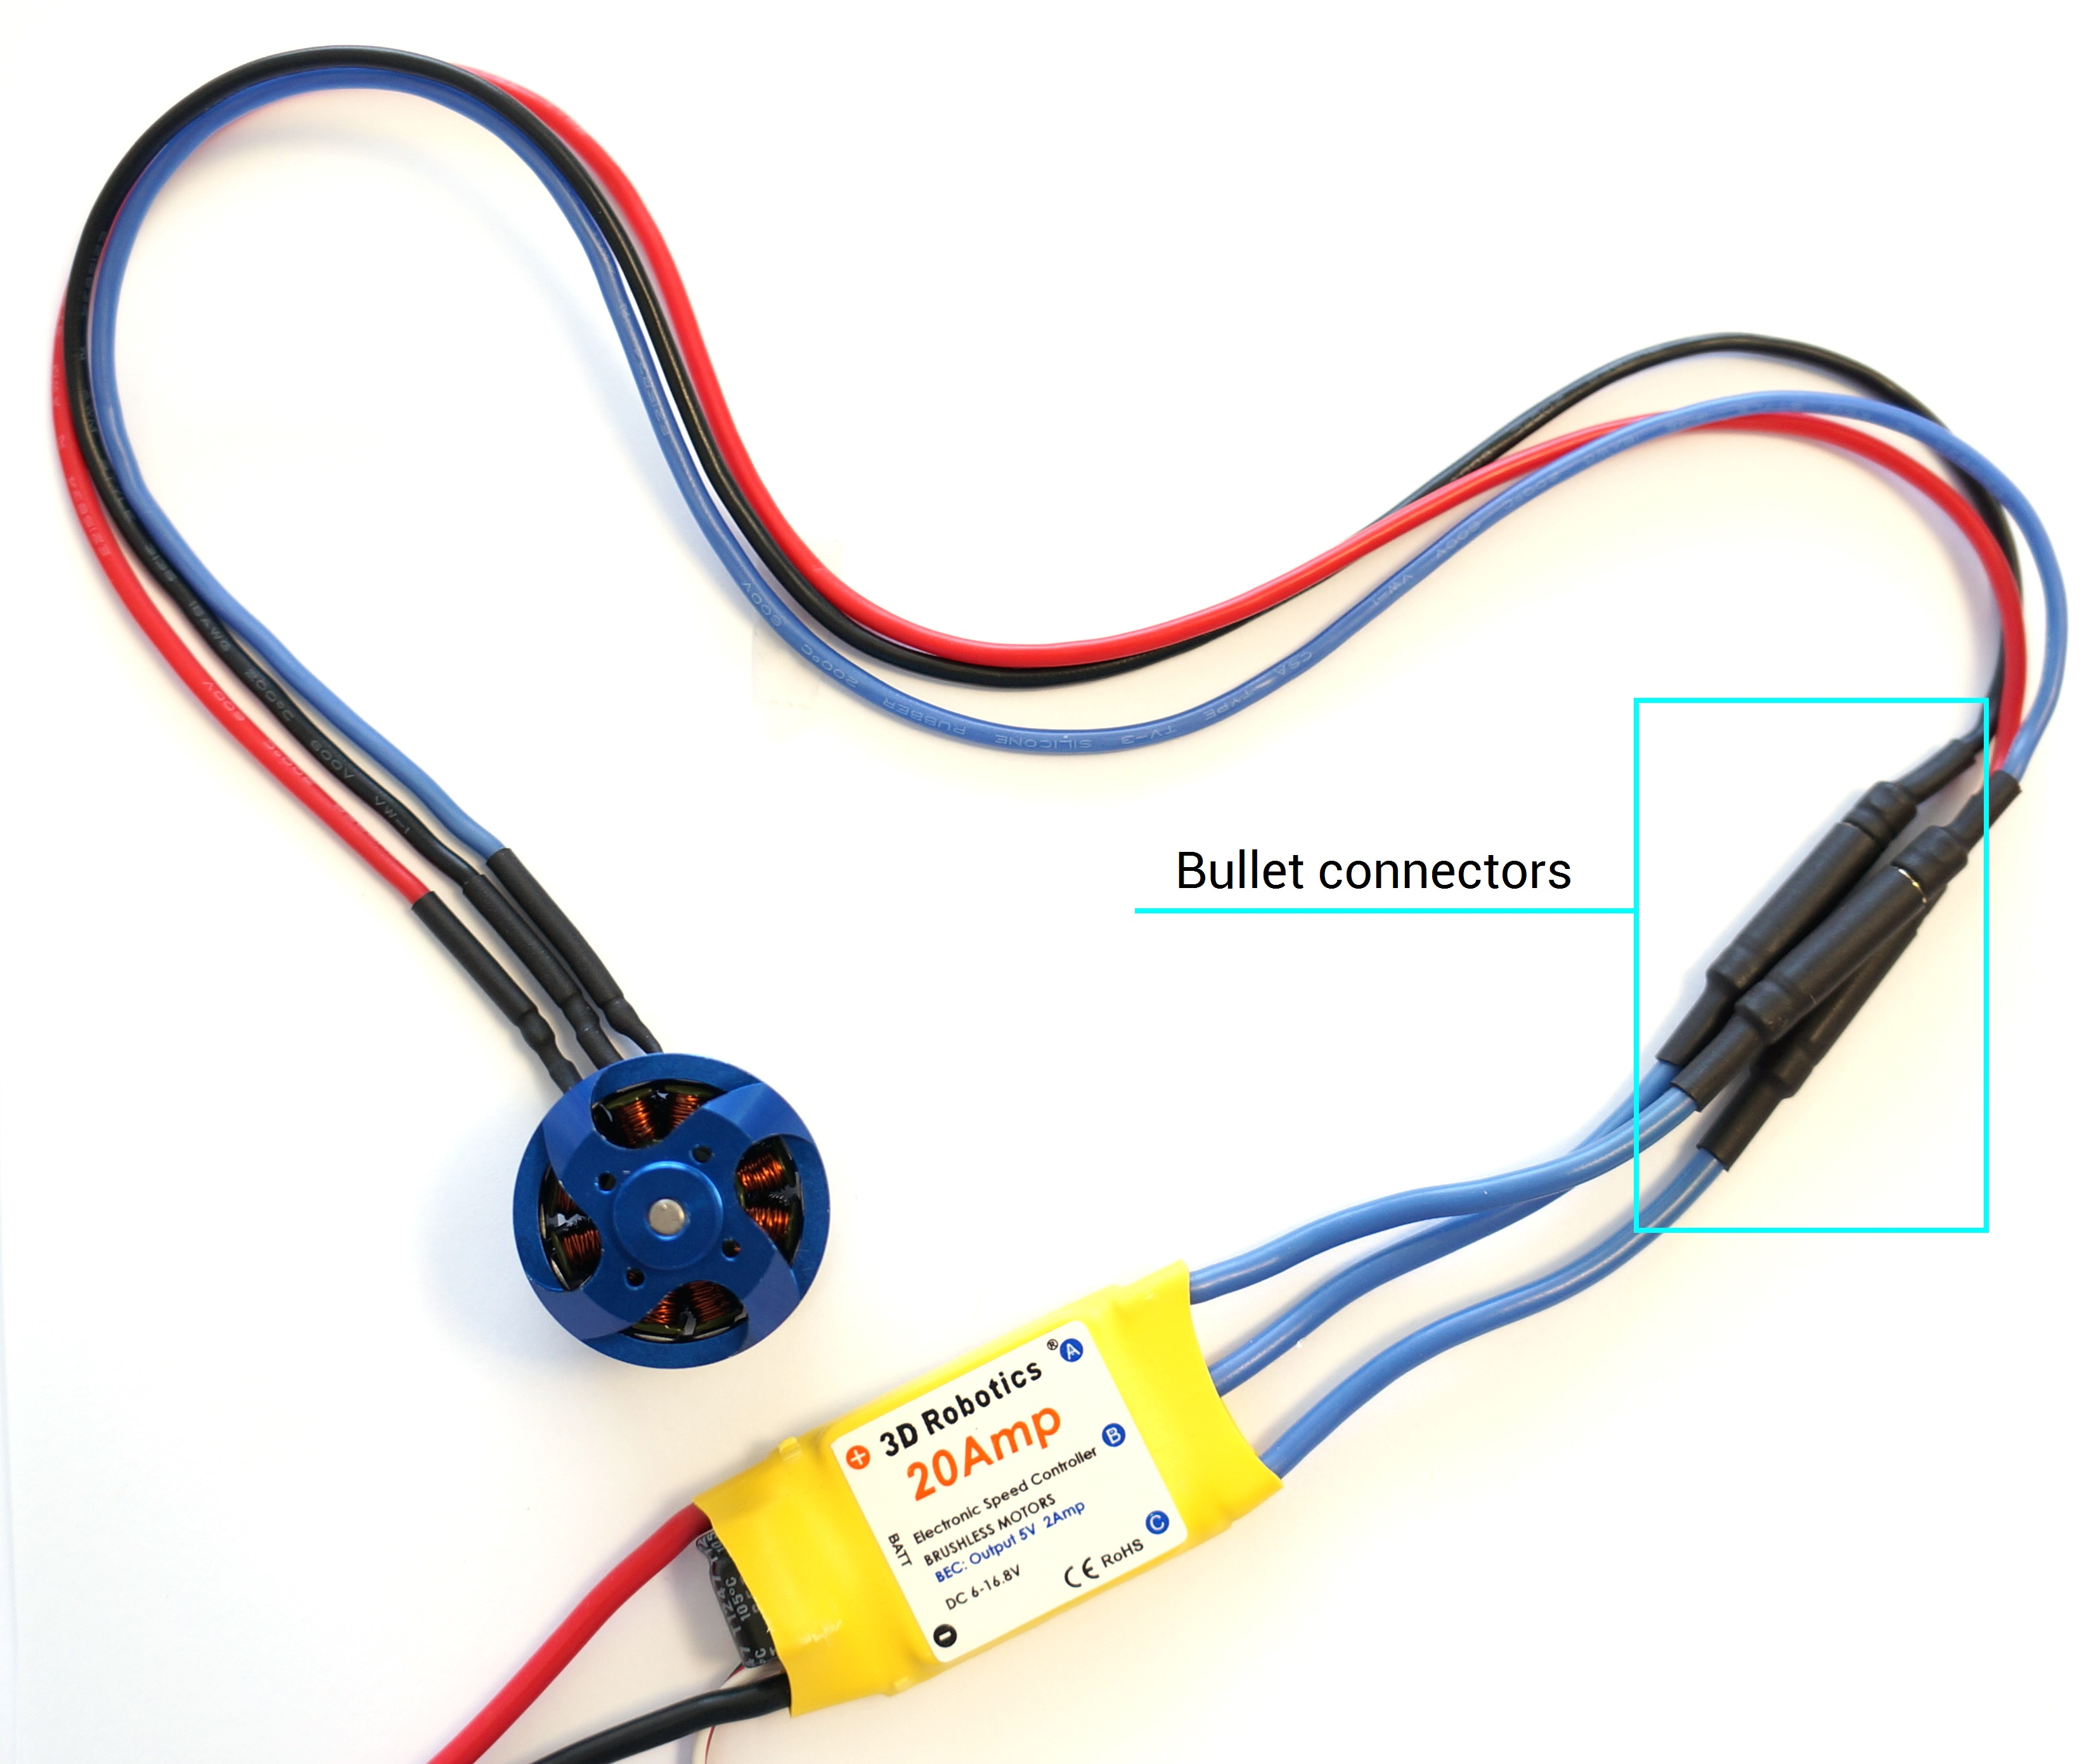
\includegraphics[width=0.7\textwidth]{Pictures/esc-motor-connect.jpg}
		%\rule{35em}{0.5pt}
	\caption[Przykładowy sterownik silnika bezszczotkowego]{Przykładowy sterownik silnika bezszczotkowego wraz z podłączonym silnikiem}
	\label{fig:esc-motor-connect.jpg}
\end{figure}


\subsection{Silniki}

Silniki wraz z przymocowanymi śmigłami zapewniają kwawdrokopterowi siłę nośną. Można je podzielić na dwie klasy: silniki bezszczotkowe i silniki szczotkowe. Silniki bezszczotkowe charakteryzują się dużą mocą i sprawnością, lecz bardzo duży pobór prądu jest ich wawdą. Silniki bezszczotkowe pobierają zdecydowanie mniej prądu niż silniki szczotkowe, lecz ich mała moc ogranicza maksymalną masę kwadrokoptera. Obecnie najczęściej stosowane są silniki bezszczotkowe, które dzięki dużej mocy umożliwiają dołączanie dodatkowych podzespołów do kwadrokoptera, takich jak moduł kamery ze stabilizacją, manipulatory, itp.

%----------------------------------------------------------------------------------------
%	SECTION 3
%----------------------------------------------------------------------------------------

\section{Konstrukcje nośne}

Konstrukcja nośna, czyli rama kwadrokoptera, stanowi platformę do mocowania wszystkich podzespołów. 

\begin{figure}[H]
	\centering
		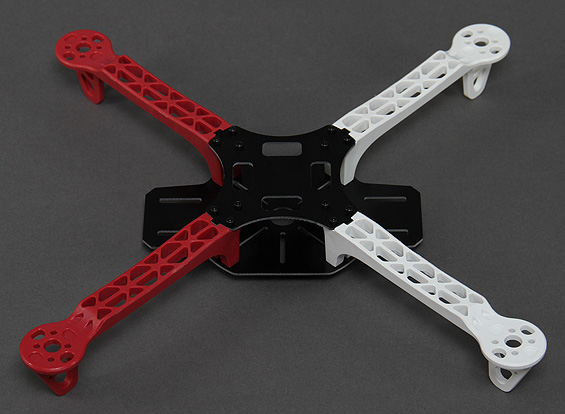
\includegraphics[width=0.7\textwidth]{Pictures/quadrotor_frame.jpg}
		%\rule{35em}{0.5pt}
	\caption[Gotowa rama do kwadrokoptera]{Gotowa rama do kwadrokoptera}
	\label{fig:quadrotor_frame.jpg}
\end{figure}

\begin{figure}[H]
	\centering
		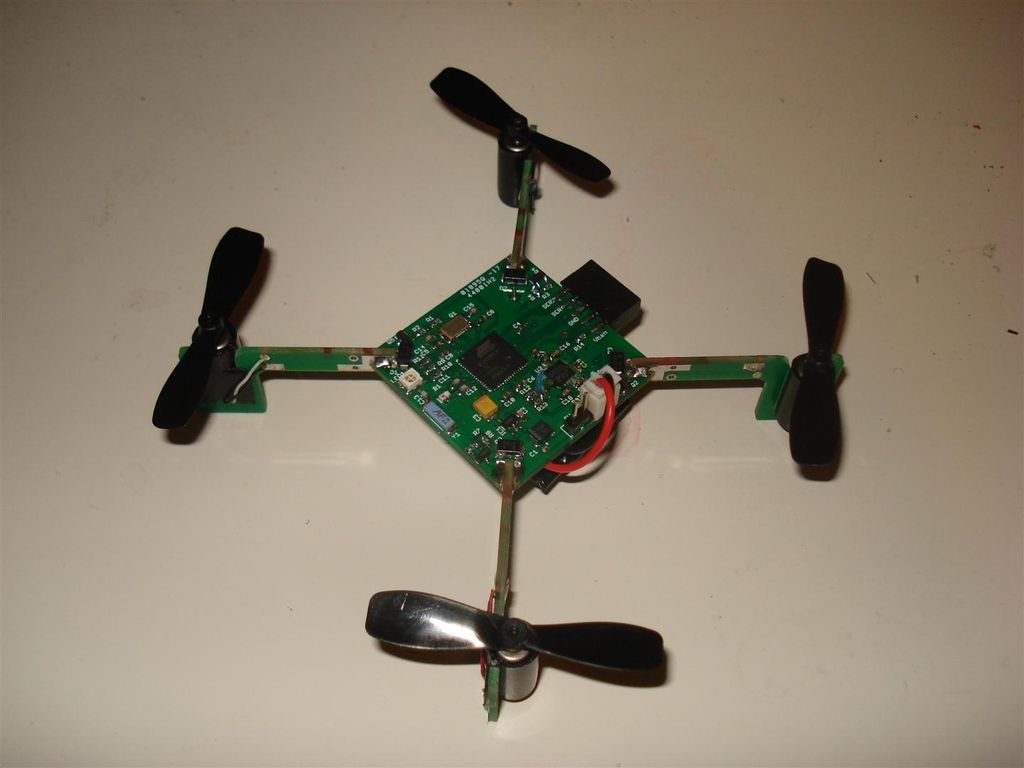
\includegraphics[width=0.7\textwidth]{Pictures/picocopter.jpg}
		%\rule{35em}{0.5pt}
	\caption[Rama kwadrokoptera zintegrowana z PCB]{Rama kwadrokoptera zintegrowana z PCB}
	\label{fig:picocopter.jpg}
\end{figure}


Ramy kwadrokopterów można podzielić na trzy główne kategorie:

\begin{itemize}
	\item Wykonana własnoręcznie
	\item Rama w postaci modułów do samodzielnego złożenia
	\item Rama zintegrowana z PCB
\end{itemize}

W przypadku wielu konstrukcji ich autorzy sami konstruują ramę, wykorzystując najczęściej takie materiały, jak aluminium lub włókno węglowe. Pozwala to dopasować projekt do swoich specyficznych potrzeb. W przypadku gdy potrzeby te nie są aż tak wyrafinowane, bardzo dobsym rozwiązaniem jest kupno gotowej ramy w formie modułów do samodzielnego złożenia (Rys.~\ref{fig:quadrotor_frame.jpg}). Dzięki takiemu rozwiązaniu omija się konieczność tworzenia całej mechaniki projektu od zera . Dla bardzo małych konstrukcji, przy których rama kwadrokoptera nie musi znosić dużych obciążeń, a jednocześnie musi być jak najlżejsza, stosuje się ramę zintegrowaną z płytką drukowaną kontrolera lotu kwadrokoptera (Rys.~\ref{fig:picocopter.jpg}). Dzięki takiemu rozwiązaniu można uzyskać bardzo niski koszt oraz masę konstrukcji. 

%----------------------------------------------------------------------------------------
%	SECTION 4
%----------------------------------------------------------------------------------------

\section{Kierunki rozwoju}

Obecnie kwadrokoptery wchodzą do coraz szerszych zastosowań. Już teraz powstają firmy specjalizujące się w zdjęciach i filmach lotniczych kręconych za pomocą kwadrokopterów. Policja tez zaczyna używać quadrocopterów. Z biegiem czasu quadrocoptery zaczną znajdować zastosowanie w coraz większej liczbie dziedzin (patrole dużych terenów, transport książek (AMAZON) itp itd) Quadrokoptery znajdują również zastosowanie w dziedzinie rozrywki - wyścigi quadrocopterów z kamerami na pokładzie.

Jeśli chodzi o rozwój quadrocopterów od strony mechanicznej coraz częściej spotykane są kontrukcje hexacopterów (6 śmigieł) oraz różne inne wariacje (Quadrokopter z jednym dużym śmigłem i trzema do manewrowania (odniesienie do bibliografii)) powstają również coraz bardziej zaawansowane algorytmy do sterowania quadrocopterami umożliwiające utrzymanie się w powietrzu nawet po utracie jednego czy dwóch wirników.
